%%% pres_quasincompact3d.tex --- 
%% 
%% Filename: pres_quasincompact3d.tex
%% Description: 
%% Author: Paul Bartholomew
%% Maintainer: 
%% Created: Wed Jan 10 10:05:43 2018 (+0000)
%% Version: 
%% Package-Requires: ()
%% Last-Updated: Tue Mar 27 23:16:14 2018 (+0100)
%%           By: Paul Bartholomew
%%     Update #: 499
%% URL: 
%% Doc URL: 
%% Keywords: 
%% Compatibility: 
%% 
%%%%%%%%%%%%%%%%%%%%%%%%%%%%%%%%%%%%%%%%%%%%%%%%%%%%%%%%%%%%%%%%%%%%%%
%% 
%%% Commentary: 
%% 
%% Talk length: 30 mins (inc. questions)
%% -> approx. 25-30 slides
%%
%% Intro:                                   TODO
%% - Outline of talk                        TODO                    1
%% - Background:                            TODO
%% --- What problem are we trying to solve? TODO                    2
%% --- What is LMN?                         TODO                    3
%% --- Outline of LMN approximation         TODO                    4
%% Numerics:                                TODO
%% - The basic numerical method             TODO                    5
%% - Treatment of Poisson equation:         TODO
%% --- Constant-coefficient                 TODO                    6
%% --- Variable-coefficient                 TODO                    7
%% --- Discussion - pros/cons               TODO                    8
%% Test-cases:                              TODO
%% - Overview                               TODO                    9
%% - 2D Mixing layer:                       TODO                   
%% --- Detailed description of case         TODO                   10
%% --- Comparison with Golanski2005         TODO                   11
%% --- Discussion                           TODO                   12
%% - Jet:                                   TODO
%% --- Detailed description of case         TODO                   13
%% --- Analysis of results                  TODO                   14
%% Conclusion + Further work                TODO                   15
%% 
%%%%%%%%%%%%%%%%%%%%%%%%%%%%%%%%%%%%%%%%%%%%%%%%%%%%%%%%%%%%%%%%%%%%%%
%% 
%%% Change Log:
%% 
%% 
%%%%%%%%%%%%%%%%%%%%%%%%%%%%%%%%%%%%%%%%%%%%%%%%%%%%%%%%%%%%%%%%%%%%%%
%% 
%% This program is free software: you can redistribute it and/or modify
%% it under the terms of the GNU General Public License as published by
%% the Free Software Foundation, either version 3 of the License, or (at
%% your option) any later version.
%% 
%% This program is distributed in the hope that it will be useful, but
%% WITHOUT ANY WARRANTY; without even the implied warranty of
%% MERCHANTABILITY or FITNESS FOR A PARTICULAR PURPOSE.  See the GNU
%% General Public License for more details.
%% 
%% You should have received a copy of the GNU General Public License
%% along with GNU Emacs.  If not, see <http://www.gnu.org/licenses/>.
%% 
%%%%%%%%%%%%%%%%%%%%%%%%%%%%%%%%%%%%%%%%%%%%%%%%%%%%%%%%%%%%%%%%%%%%%%
%% 
%%% Code:

\documentclass[
linkcolor=red,
urlcolor=blue
]{beamer}

\usepackage{graphicx}
\usepackage{subfigure}
\usepackage{natbib}
\usepackage{tikz}
\usepackage{pgfplots}
\usepackage{nicefrac}
\usepackage{epstopdf}
\usepackage{booktabs}
% \usepackage{media9}
% \usepackage{movie15}
\usepackage{multimedia}

\setbeamertemplate{itemize items}[circle]

\newcommand{\quasincompact}{\texttt{QuasIncompact3D}}
\newcommand{\incompact}{\texttt{Incompact3D}}

\newcommand{\dtrans}[1]{\frac{d#1}{dt}}
\newcommand{\Dtrans}[1]{\frac{D#1}{Dt}}
\newcommand{\vvect}[1]{\boldsymbol{#1}}
\newcommand{\vdiv}[1]{\vvect{\nabla} \cdot #1}
\newcommand{\vgrad}[1]{\vvect{\nabla} #1}
\newcommand{\density}{\rho}
\newcommand{\velocity}{u}
\newcommand{\vvelocity}{\vvect{\velocity}}
\newcommand{\pressure}{p}
\newcommand{\viscstress}{\tau}
\newcommand{\vviscstress}{\vvect{\tau}}
\newcommand{\temperature}{T}
\newcommand{\Reynolds}{Re}
\newcommand{\Prandtl}{Pr}
\newcommand{\visc}{\mu}
\newcommand{\identity}{I}
\newcommand{\poissiter}{\nu}
\newcommand{\massfrac}{Y}
\newcommand{\Schmidt}{Sc}
\newcommand{\diffcoeff}{\mathcal{D}}

\newcommand{\subrule}{\vspace{0.1cm}\hrule}

\title{Simulations of Variable-Density Flows in the Low Mach Number Limit}
\author{Paul Bartholomew\\Sylvain Laizet}
\date{March 28, 2018\\\vspace{0.5cm}\incompact\ User Group Meeting}

\begin{document}

% Title page
\begin{frame}
  \thispagestyle{empty}
  \titlepage
\end{frame}

%%%%%%%%%%%%%%%%%%%%%%%%%%%%%%%%%%%%%%%%%%%%%%%%%%%%%%%%%%%%%%%%%%%%%%
%% Introduction

% Introduction page
\begin{frame}
  \frametitle{Introduction}
  \framesubtitle{Outline\subrule}

  \begin{itemize}
  \item Introduction
    \begin{itemize}
    \item Motivation
    \item The Low Mach Number (LMN) approximation
    \end{itemize}
  \item \quasincompact:\ the implementation of LMN in \incompact
    \begin{itemize}
    \item Algorithm to solve LMN
    \item Treatment of pressure equation
    \end{itemize}
  \item Testcases
    \begin{itemize}
    \item 2D mixing layer
    \item Jet
    \end{itemize}
  \item Conclusion
  \end{itemize}
\end{frame}

\begin{frame}
  \frametitle{Introduction}
  \framesubtitle{What problem are we trying to solve?\subrule}

  % As the title says, what problem are we trying to solve?
  \begin{itemize}
  \item \incompact\ provides powerful capabilities for solving \textit{incompressible} flows\ldots
  \item or flows with small density variations
  \end{itemize}
  \begin{figure}[h]
    \centering
    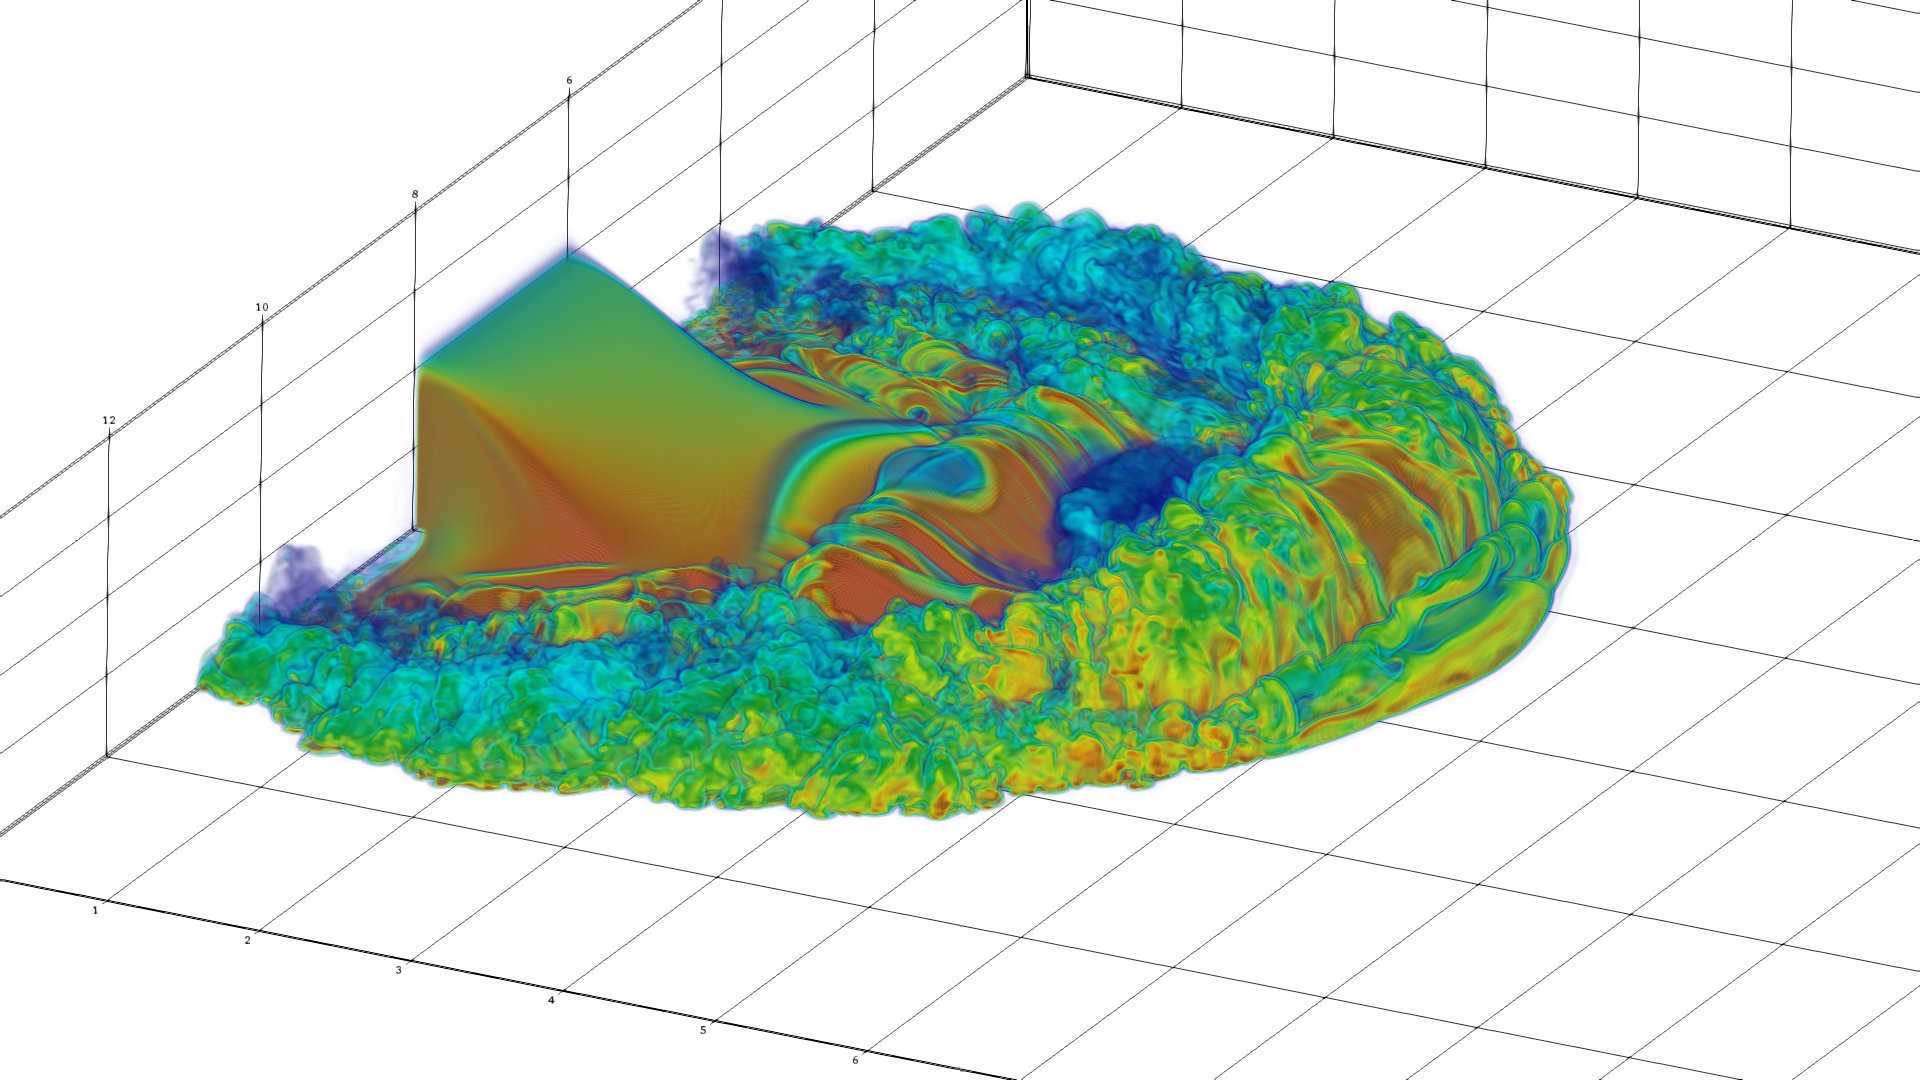
\includegraphics[width=0.675\textwidth]{./figures/gravity-driven_particles}
    \caption{Gravity-driven flow simulated by
      \incompact\footnote{\url{https://twitter.com/incompact3d}}}\label{fig:grav-driven}
  \end{figure}
\end{frame}

\begin{frame}
  \frametitle{Introduction}
  \framesubtitle{The problem with compressible flow\subrule}
  \begin{itemize}
  \item If density variations are significant, needs to be treated as \textit{compressible} flow
  \item Flow velocity may still be low ($\gamma M^2 \ll 1$)
  \item Results in ill-conditioned equations, \textit{e.g.}
    \begin{equation*}
      \gamma M^2 \density \Dtrans{\vvelocity} = -\vgrad{\pressure} + \frac{\gamma M^2}{\Reynolds}
      \vdiv{\vviscstress}
    \end{equation*}
  \item Numerically this leads to requirement for very small timesteps
    \begin{itemize}
    \item[\textcolor{red}{\textbf{--}}] Inefficient!
    \end{itemize}
  \end{itemize}
\end{frame}

\begin{frame}
  \frametitle{Introduction}
  \framesubtitle{The Low Mach Number Approximation\subrule}
  \begin{itemize}
  \item Expand variables as power series using $\varepsilon = \gamma M^2$ as the small parameter
    and take lowest order terms (recall $\gamma M^2 \ll 1$)
    \begin{equation*}
      \vvelocity = \vvelocity^{\left( 0 \right)} + \varepsilon \vvelocity^{\left( 1 \right)} +
      \varepsilon^2 \vvelocity^{\left( 2 \right)} + \ldots
    \end{equation*}
  \end{itemize}
  \begin{align*}
    % EOS
    \pressure^{\left( 0 \right)} &= \density^{\left( 0 \right)} \temperature^{\left( 0 \right)}
    % \frac{\mathcal{R}}{\overline{W}}
    \\
    % Continuity
    \frac{\partial \density^{\left( 0 \right)}}{\partial t} + \vdiv{\density^{ \left( 0 \right)}
    \vvelocity^{\left( 0 \right)}} &= 0 \\
    % Lowest order momentum: grad(p^0) = 0
    \vvect{0} &= \vgrad{\pressure^{\left( 0 \right)}} \\
    % Energy/temperature equation
    \density^{\left( 0 \right)} \frac{\partial \temperature^{\left( 0 \right)}}{\partial t} +
    \density^{\left( 0 \right)} \vvelocity^{\left( 0 \right)} \cdot \vgrad{\temperature^{\left( 0
    \right)}} &= \frac{\vdiv{k \vgrad{\temperature^{\left( 0
                \right)}}}}{\Reynolds\Prandtl\temperature^{\left( 0 \right)}} + \dtrans{p^{\left( 0
                \right)}} \\
    % Mass-fraction transport
    % \density^{\left( 0 \right)} \frac{\partial \massfrac}{\partial t} + \density^{\left( 0 \right)}
    % \vvelocity^{\left( 0 \right)} \cdot \vgrad{\massfrac} &= \frac{\vdiv{\density^{\left( 0 \right)}
    %                                                         \diffcoeff \vgrad{\massfrac}}}{\Reynolds
    %                                                         \Schmidt} \\
    % Momentum equation
    \frac{\partial \density^{\left( 0 \right)} \vvelocity^{\left( 0 \right)}}{\partial t} +
    \vdiv{\density^{\left( 0 \right)} \vvelocity^{\left( 0 \right)} \vvelocity^{\left( 0 \right)}}
                                   &= - \vgrad{\pressure^{\left( 1 \right)}} +
                                     \frac{\vdiv{\vviscstress^{\left( 0 \right)}}}{\Reynolds}
    \end{align*}
\end{frame}
\begin{frame}
  \frametitle{Introduction}
  \framesubtitle{The Low Mach Number Approximation (cont.)\subrule}

  \begin{itemize}
  \item Combining continuity and temperature equations yields velocity divergence constraint
    \begin{equation*}
      \vdiv{\vvelocity} = \frac{1}{\pressure^{\left( 0 \right)}} \left( \frac{\vdiv{k
            \vgrad{\temperature}}}{\Reynolds \Prandtl} - \dtrans{\pressure^{\left( 0 \right)}}
      \right)
    \end{equation*}
  \item Boundary condition follows
    \begin{equation*}
      \int_{\partial \Omega} \vvelocity \cdot \widehat{\vvect{n}} dS = \frac{1}{\pressure^{\left( 0
          \right)}} \left( \frac{1}{\Reynolds \Prandtl} \int_{\partial \Omega} k
        \vgrad{\temperature} \cdot \widehat{\vvect{n}} dS - \dtrans{\pressure^{\left( 0 \right)}}
        V_{\Omega} \right)
    \end{equation*}
  \item Open domains
    \begin{equation*}
      \dtrans{\pressure^{\left( 0 \right)}} = 0 \Rightarrow \pressure^{\left( 0 \right)} = \pressure_a
    \end{equation*}
  \end{itemize}
\end{frame}

%%%%%%%%%%%%%%%%%%%%%%%%%%%%%%%%%%%%%%%%%%%%%%%%%%%%%%%%%%%%%%%%%%%%%%
%% Numerics
\begin{frame}
  \frametitle{Numerical Method}
  \framesubtitle{Overview\subrule}

  \begin{itemize}
  \item Advance density in time
    \begin{equation*}
      \density^{k+1} = \density^k + \Delta t \vdiv{{\left( \density \vvelocity \right)}^k}
    \end{equation*}
  \item Update temperature via EOS and compute $\vdiv{\vvelocity}^{k+1}$
    \begin{equation*}
      \temperature^{k+1} = \frac{\pressure^{\left( 0 \right)}}{\density^{k+1}} \Rightarrow
      \vdiv{\vvelocity^{k+1}} = \frac{\vdiv{k \vgrad{ T^{k+1}}}}{p^{\left( 0 \right)} \Reynolds
        \Prandtl}
    \end{equation*}
  \item Integrate momentum via fractional step method\footnote{\citet{Chorin1997}}
    \begin{align*}
      {\left( \density \vvelocity \right)}^{\star} &= {\left( \density \vvelocity \right)}^k -
                                                     \Delta t \left( \vdiv{{\left( \density
                                                     \vvelocity \vvelocity \right)}^k} -
                                                     \frac{\vdiv{\vviscstress^k}}{\Reynolds} \right)
      \\
      {\left( \density \vvelocity \right)}^{k+1} &= {\left( \density \vvelocity \right)}^{\star} -
                                                   \Delta t \vgrad{\widetilde{\pressure^{\left( 1
                                                   \right)}}^{k+1}} \Rightarrow \vvelocity^{k+1} =
                                                   \frac{{\left( \density \vvelocity
                                                   \right)}^{k+1}}{\density^{k+1}}
    \end{align*}
  \end{itemize}
\end{frame}

\begin{frame}
  \frametitle{Numerical Method}
  \framesubtitle{The Poisson Equation - Constant Coefficient\subrule}

  \begin{itemize}
  \item Like incompressible approach, take divergence of momentum directly
    \begin{equation*}
      {\nabla}^2 \widetilde{\pressure^{\left( 1 \right)}}^{k+1} = \frac{1}{\Delta t} \left(
        \vdiv{{\left( \density \vvelocity \right)}^{\star}} - \vdiv{{\left( \density \vvelocity
            \right)}^{k+1}}
      \right)
    \end{equation*}
  \item[\textcolor{blue}{\textbf{+}}] Constant coefficient Poisson equation: direct solution
    possible
  \item[\textcolor{red}{\textbf{--}}] Need an approximation for $\vdiv{{\left( \density \vvelocity
        \right)}^{k+1}}$
    \begin{equation*}
      \vdiv{{\left( \density \vvelocity \right)}^{k+1}} = - \left. \frac{\partial
          \density}{\partial t} \right|^{k+1} \approx -\frac{\density^{k+1} - \density^k}{\Delta t}
    \end{equation*}
  \end{itemize}
\end{frame}

\begin{frame}
  \frametitle{Numerical Method}
  \framesubtitle{The Poisson Equation - Variable Coefficient\subrule}

  \begin{itemize}
  \item Alternatively, $\vdiv{\vvelocity^{k+1}}$ is available as a
    constraint\footnote{\textit{c.f.} incompressible flow: $\vdiv{\vvelocity} = 0$}
    \begin{equation*}
      \vdiv{\frac{1}{\density} \vgrad{\widetilde{p^{\left( 1 \right)}}^{k+1}}} = \frac{1}{\Delta t}
      \left( \vdiv{\vvelocity^{\star}} - \vdiv{\vvelocity^{k+1}} \right)
    \end{equation*}
  \item Cannot solve directly using FFT solver
  \item Iterative solver
  \end{itemize}
  \begin{align*}
    {\nabla}^2 \widetilde{\pressure^{\left( 1 \right)}}^{\poissiter+1} &= {\nabla}^2
                                                                         \widetilde{\pressure^{\left(
                                                                         1 \right)}}^{\poissiter}
                                                                         + \widetilde{\density}
                                                                         \left[ \frac{1}{\Delta t}
                                                                         \left(
                                                                         \vdiv{\vvelocity^{\star}}
                                                                         -
                                                                         \vdiv{\vvelocity^{k+1}}\right)
                                                                         -
                                                                         \vdiv{\frac{1}{\density}
                                                                         \vgrad{\widetilde{\pressure^{\left(
                                                                         1 \right)}}^{\poissiter}}}
                                                                         \right] \\
                                                                       & \left|\left| \Delta
                                                                         \widetilde{\pressure^{\left(
                                                                         1 \right)}} \right|\right|
                                                                         \leq \texttt{tol}
    \end{align*}
\end{frame}

\begin{frame}
  \frametitle{Numerical Method}
  \framesubtitle{The Poisson Equation - Variable Coefficient, Choice of
    $\widetilde{\density}$\subrule}

  \begin{itemize}
  \item Free choice of $\widetilde{\density}$
  \item Choice of $\widetilde{\density}$ will affect convergence
  \item Typical choices are an average or minimum value, $\widetilde{\density} = \density_0$
    \begin{itemize}
    \item Stems from `\textit{brute force}' derivation of iteration equation
    \end{itemize}
  \item Chain-rule suggests $\widetilde{\density}$ should vary in space
    \begin{equation*}
      \begin{split}
        \vdiv{\frac{1}{\density} \vgrad{\widetilde{\pressure^{\left( 1 \right)}}}} &=
        \frac{1}{\density} {\nabla}^2 \widetilde{\pressure^{\left( 1 \right)}} +
        \vgrad{\frac{1}{\density}} \cdot \vgrad{\widetilde{\pressure^{\left( 1 \right)}}} \\
        &= \frac{1}{\density} {\nabla}^2 \widetilde{\pressure^{\left( 1 \right)}} + \left(
          \vdiv{\frac{1}{\density} \vgrad{\widetilde{\pressure^{\left( 1 \right)}}}} -
          \frac{1}{\density} {\nabla}^2 \widetilde{\pressure^{\left( 1 \right)}} \right) \\
        \Rightarrow \widetilde{\density} &= {\left( \overline{\nicefrac{1}{\density}} \right)}^{-1}
      \end{split}
    \end{equation*}
  \item[\textcolor{blue}{\textbf{+}}] Harmonic average is proportional to local minimum
  \end{itemize}
\end{frame}

\begin{frame}
  \frametitle{Numerical Method}
  \framesubtitle{The Poisson Equation - Discussion\subrule}

  \begin{itemize}
    \setlength{\itemsep}{0.4cm}
  \item \textbf{Constant coefficient}
    \begin{itemize}
      \setlength{\itemsep}{0.25cm}
    \item[\textcolor{blue}{\textbf{+}}] Direct solver $\rightarrow$ fast solution
    \item[\textcolor{red}{\textbf{--}}] Extrapolation is potential source of error
    \item[\textcolor{red}{\textbf{--}}] Does not recover $\vdiv{\vvelocity}^{k+1} = 0$ in inviscid
      case\footnote{\citet{Nicoud2000}}
    \end{itemize}
  \item \textbf{Variable coefficient}
    \begin{itemize}
      \setlength{\itemsep}{0.25cm}
    \item[\textcolor{blue}{\textbf{+}}] Obeys $\vdiv{\vvelocity}^{k+1}$ constraint
    \item[\textcolor{red}{\textbf{--}}] Iteration is potentially very expensive!
    \end{itemize}
  \end{itemize}
\end{frame}

% %%%%%%%%%%%%%%%%%%%%%%%%%%%%%%%%%%%%%%%%%%%%%%%%%%%%%%%%%%%%%%%%%%%%%%
% %% Testcases

% \begin{frame}
%   \frametitle{Testcases}
%   \framesubtitle{Overview\subrule}

%   \begin{itemize}
%   \item 2D non-isothermal mixing layer
%   \item 3D buoyant turbulent jets
%     \begin{itemize}
%     \item Non-isothermal
%     \item Multicomponent
%     \end{itemize}
%   \end{itemize}
% \end{frame}

% 2D Non-isothermal mixing layer
\begin{frame}
  \frametitle{Testcases}
  \framesubtitle{2D Non-Isothermal Mixing Layer - Initial \& Boundary Conditions\subrule}
  \begin{columns}
    \begin{column}{0.6\textwidth}
      \begin{itemize}
      \item Hyperbolic tangent velocity profile
        \begin{equation*}
          \begin{split}
            \velocity \left( y \right) &= \frac{\velocity_1 + \velocity_2}{2} + \frac{\velocity_1 -
              \velocity_2}{2} \tanh \left( \frac{2 y}{\delta} \right) \\
            \velocity_c &= \frac{\velocity_1 \sqrt{\temperature_2} + \velocity_2
              \sqrt{\temperature_1}}{\sqrt{\temperature_1} + \sqrt{\temperature_2}} = 0 \\
            \frac{\temperature_2}{\temperature_1} &= \frac{1}{2} \ , \dtrans{p^{\left( 0 \right)}} = 0
          \end{split}
        \end{equation*}
      \item Initial perturbation applied to velocity field to promote
        transition%\footnote{See~\citet{Golanski2005}}
      \item Periodic in $x$ no-slip on $y$
      \end{itemize}
    \end{column}
    \begin{column}{0.4\textwidth}
      \begin{figure}[c]
        \centering
        %%% nonisotherm_initcond.tex --- 
%% 
%% Filename: nonisotherm_initcond.tex
%% Description: 
%% Author: Paul Bartholomew
%% Maintainer: 
%% Created: Mon Mar 12 12:26:52 2018 (+0000)
%% Version: 
%% Package-Requires: ()
%% Last-Updated: Tue Mar 13 14:37:45 2018 (+0000)
%%           By: Paul Bartholomew
%%     Update #: 52
%% URL: 
%% Doc URL: 
%% Keywords: 
%% Compatibility: 
%% 
%%%%%%%%%%%%%%%%%%%%%%%%%%%%%%%%%%%%%%%%%%%%%%%%%%%%%%%%%%%%%%%%%%%%%%
%% 
%%% Commentary: 
%% 
%% 
%% 
%%%%%%%%%%%%%%%%%%%%%%%%%%%%%%%%%%%%%%%%%%%%%%%%%%%%%%%%%%%%%%%%%%%%%%
%% 
%%% Change Log:
%% 
%% 
%%%%%%%%%%%%%%%%%%%%%%%%%%%%%%%%%%%%%%%%%%%%%%%%%%%%%%%%%%%%%%%%%%%%%%
%% 
%% This program is free software: you can redistribute it and/or modify
%% it under the terms of the GNU General Public License as published by
%% the Free Software Foundation, either version 3 of the License, or (at
%% your option) any later version.
%% 
%% This program is distributed in the hope that it will be useful, but
%% WITHOUT ANY WARRANTY; without even the implied warranty of
%% MERCHANTABILITY or FITNESS FOR A PARTICULAR PURPOSE.  See the GNU
%% General Public License for more details.
%% 
%% You should have received a copy of the GNU General Public License
%% along with GNU Emacs.  If not, see <http://www.gnu.org/licenses/>.
%% 
%%%%%%%%%%%%%%%%%%%%%%%%%%%%%%%%%%%%%%%%%%%%%%%%%%%%%%%%%%%%%%%%%%%%%%
%% 
%%% Code:

\resizebox{\columnwidth}{0.5\textheight}
{
  \begin{tikzpicture}
    \begin{axis}[
      xmin = -1.5, xmax = 1.5,
      ymin = -2, ymax = 2,
      axis lines = center,
      xlabel = $x$,
      ylabel = $y$,
      xticklabels={,,},
      yticklabels={,,}
      ]
      
      \addplot [mark = none]
      table [x=x, y=y, col sep=comma] {figures/atanhx.csv};
      
      \draw [->, thick] (axis cs: 0, 1.5) -- (axis cs: 1, 1.5);
      \node at (axis cs: 1.25, 1.5) {$\velocity_1$};
      \draw [->, thick] (axis cs: 0, -1.5) -- (axis cs: -1, -1.5);
      \node at (axis cs: -1.25, -1.5) {$\velocity_2$};
      
      \draw [dashed] (axis cs: 0, 0) -- (axis cs: 1.2, 0.66);
      \draw [<->] (axis cs: 1, 0) -- (axis cs: 1, 0.55);
      \node at (axis cs: 1.1, 0.25) {$\delta$};
      
      \node at (axis cs: -1, 1) {$\temperature_1$};
      \node at (axis cs: 1, -1) {$\temperature_2$};
    \end{axis}
  \end{tikzpicture}
}

%%%%%%%%%%%%%%%%%%%%%%%%%%%%%%%%%%%%%%%%%%%%%%%%%%%%%%%%%%%%%%%%%%%%%%
%%% nonisotherm_initcond.tex ends here

%%% Local Variables:
%%% mode: latex
%%% TeX-master: "../pres_quasincompact3d"
%%% End:

        \caption{Diagram of non-isothermal mixing layer}\label{fig:non-iso_init-cond}
      \end{figure}
    \end{column}
  \end{columns}
\end{frame}

\begin{frame}
  \frametitle{Testcases}
  \framesubtitle{2D Non-Isothermal Mixing Layer - Results (Vorticity)\subrule}

  \begin{tabular}{c c c c}
    % constcoeff - varcoeff-rho0 - varcoeff-rhoh - Golanski2005
    \textbf{CC} & \textbf{VC $\density_0$} & \textbf{VC $\density_h$} & \textbf{G2005} \\
    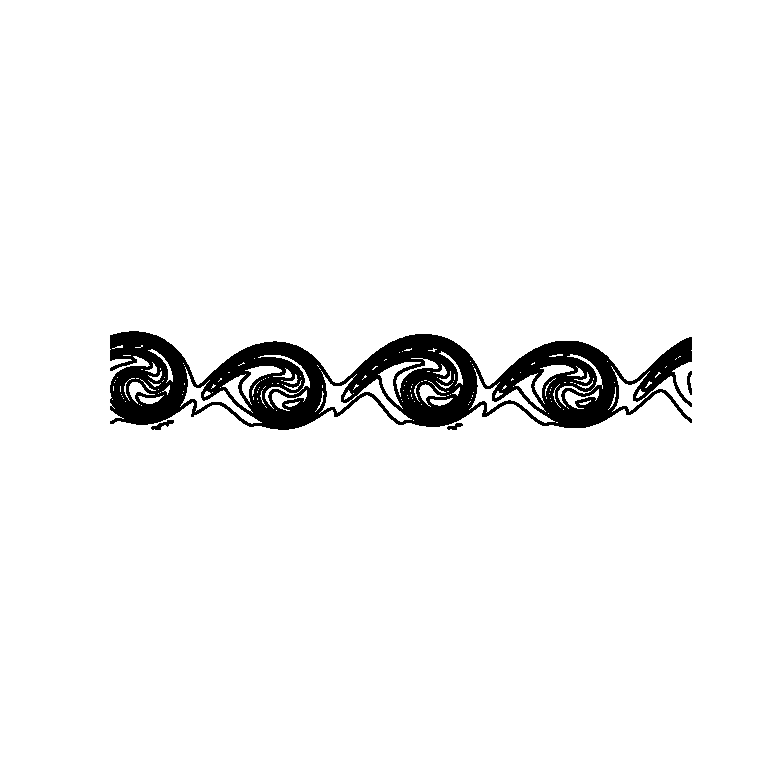
\includegraphics[width=0.225\textwidth]{figures/constcoeff-vortz-024} & 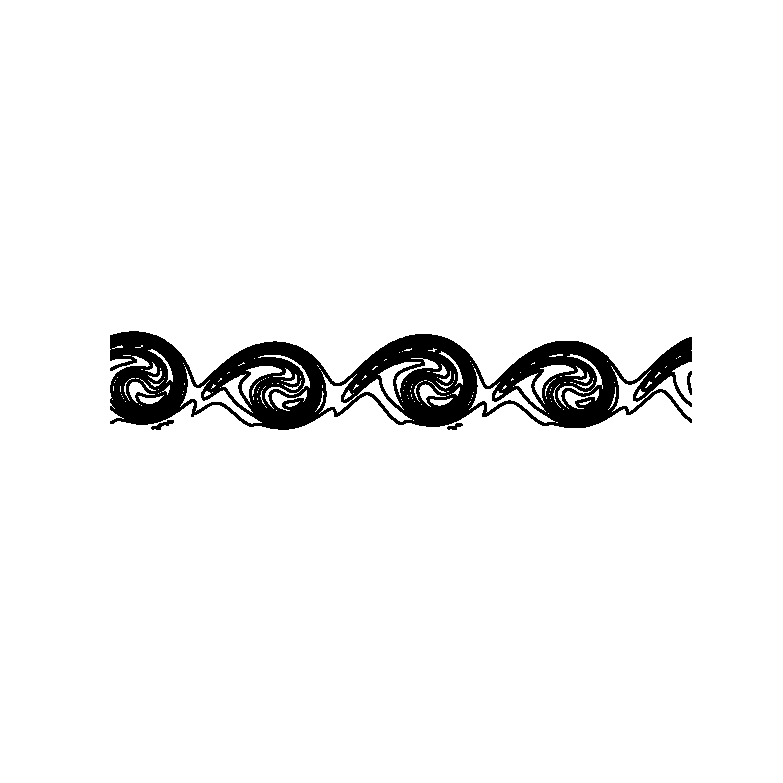
\includegraphics[width=0.225\textwidth]{figures/varcoeff-rho0-vortz-024} & 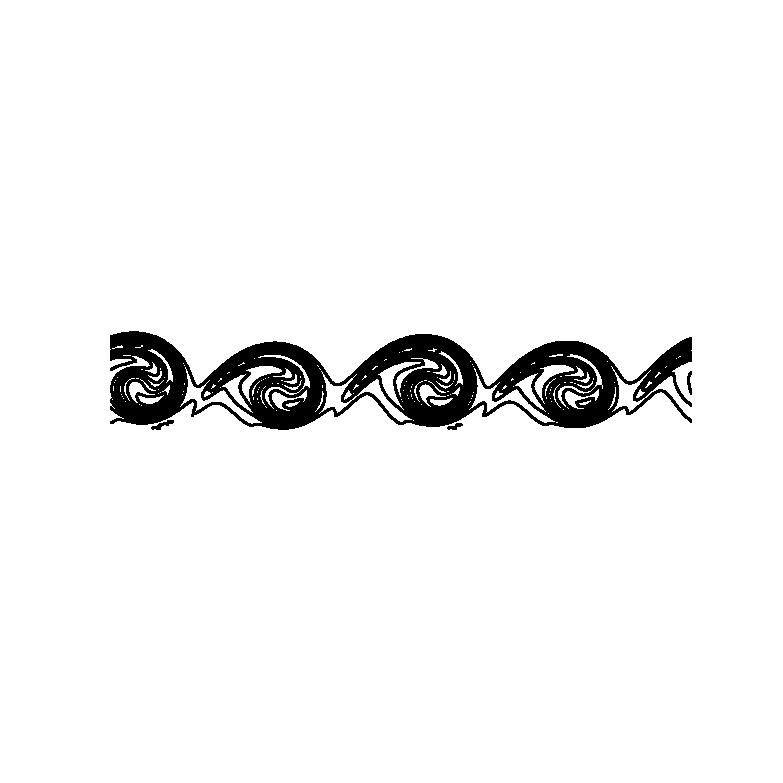
\includegraphics[width=0.225\textwidth]{figures/varcoeff-rhoh-vortz-024} & 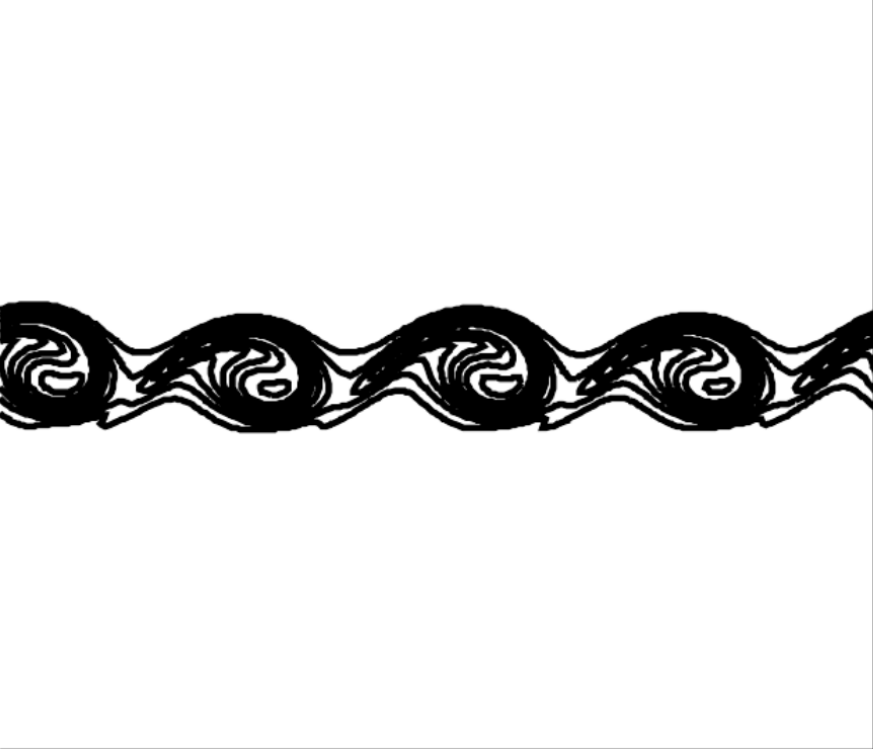
\includegraphics[width=0.225\textwidth]{figures/golanski2005-t24}
    \\
    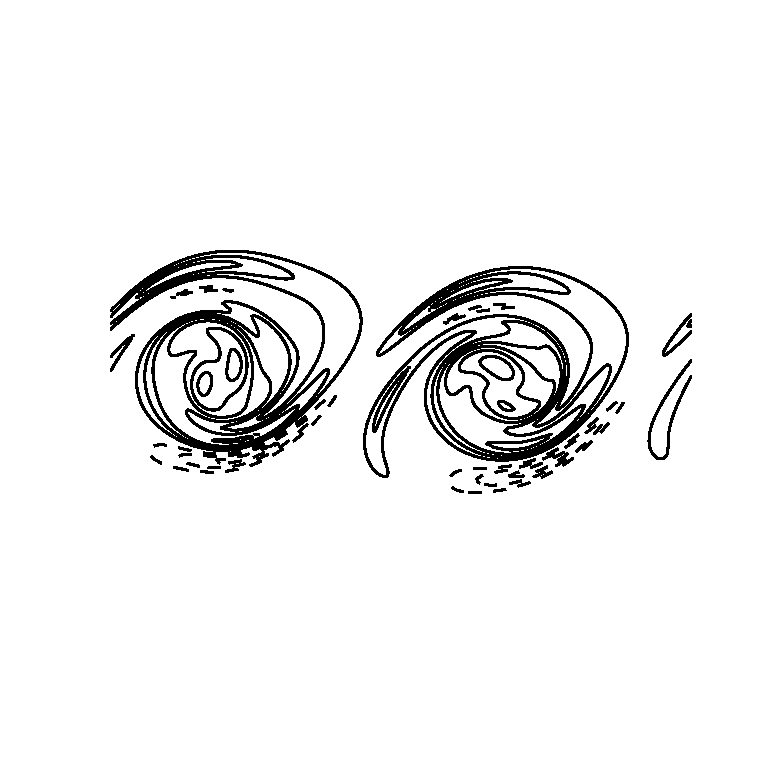
\includegraphics[width=0.225\textwidth]{figures/constcoeff-vortz-082} & 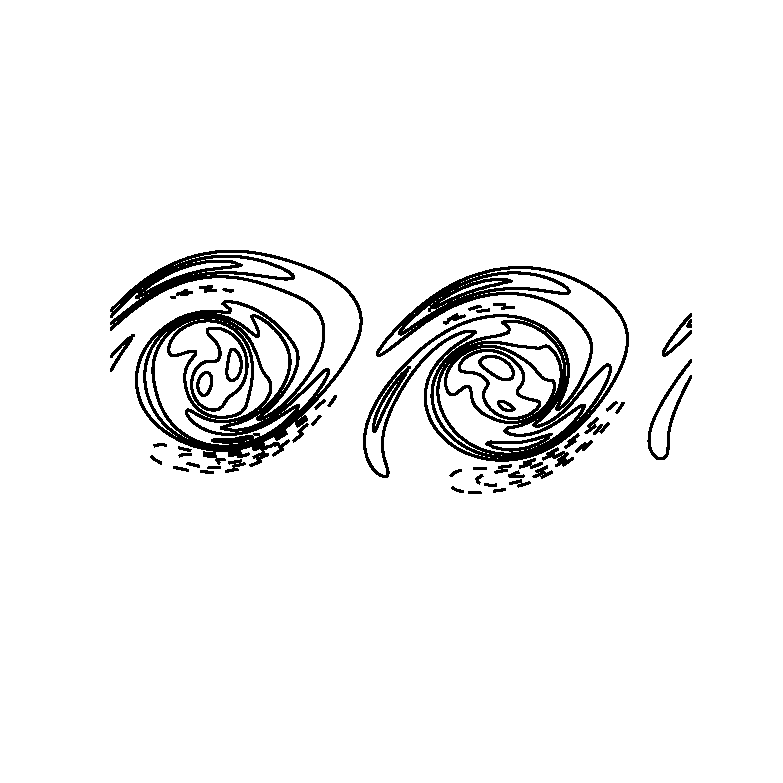
\includegraphics[width=0.225\textwidth]{figures/varcoeff-rho0-vortz-082} & 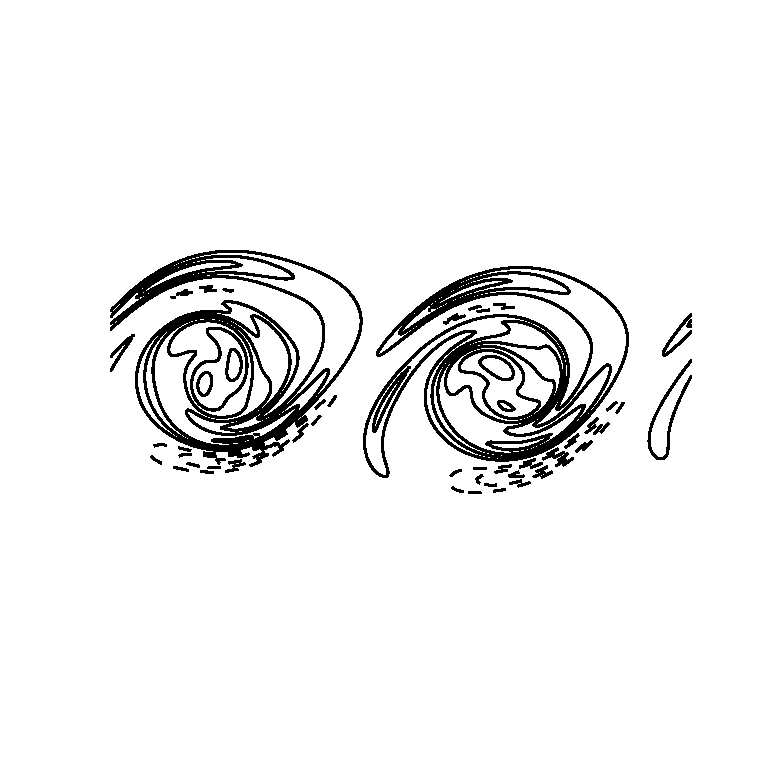
\includegraphics[width=0.225\textwidth]{figures/varcoeff-rhoh-vortz-082} &
                                                                                       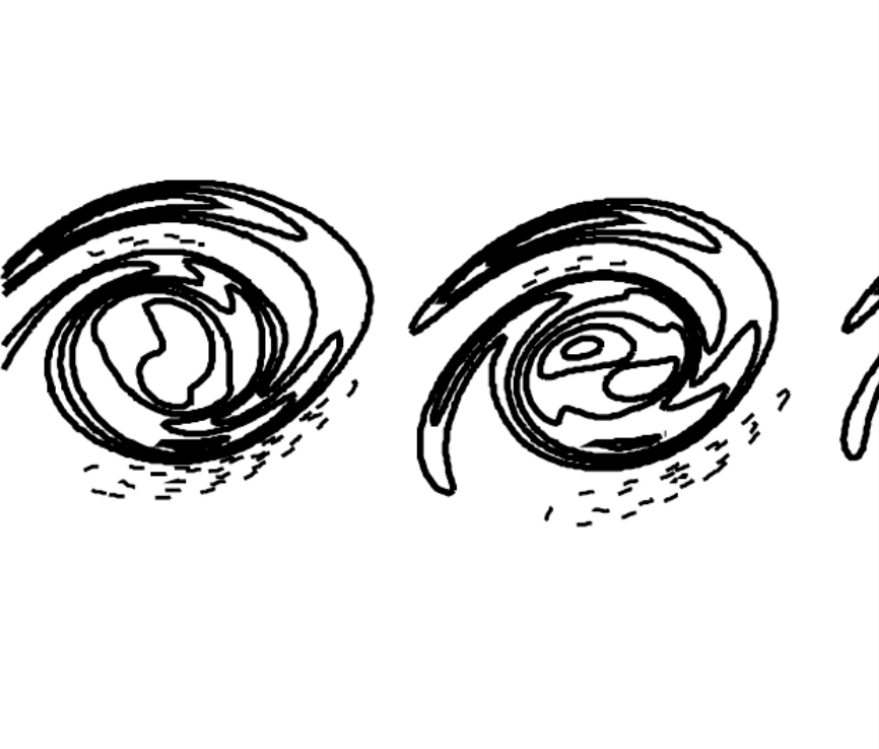
\includegraphics[width=0.225\textwidth]{figures/golanski2005-t82} \\
    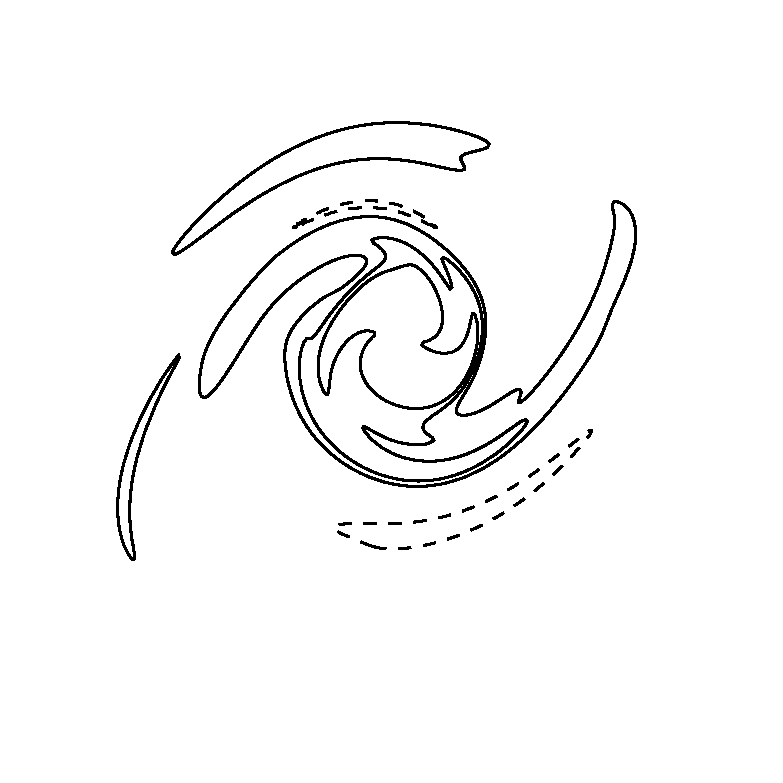
\includegraphics[width=0.225\textwidth]{figures/constcoeff-vortz-182} & 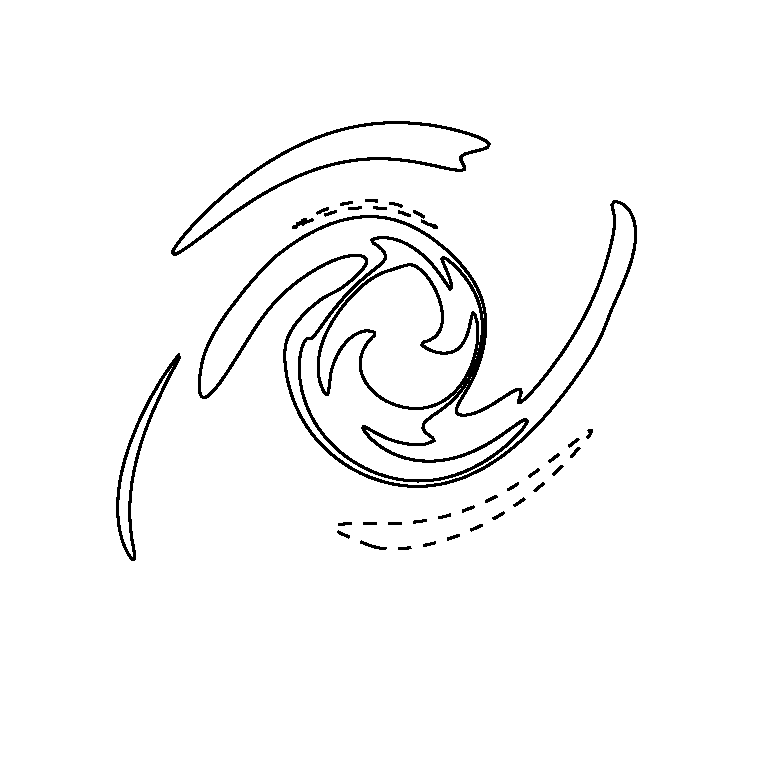
\includegraphics[width=0.225\textwidth]{figures/varcoeff-rho0-vortz-182} & 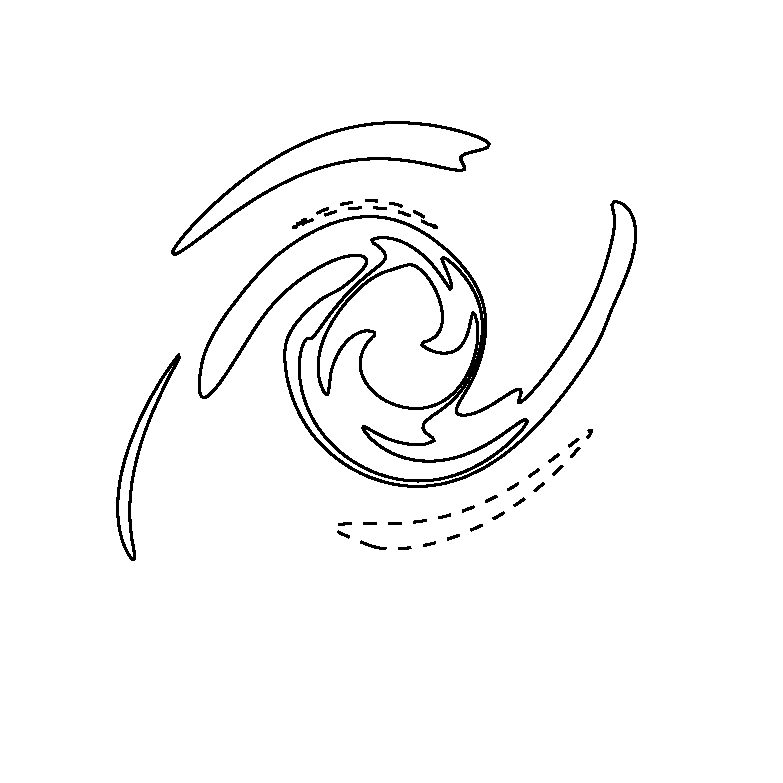
\includegraphics[width=0.225\textwidth]{figures/varcoeff-rhoh-vortz-182} &
                                                                                       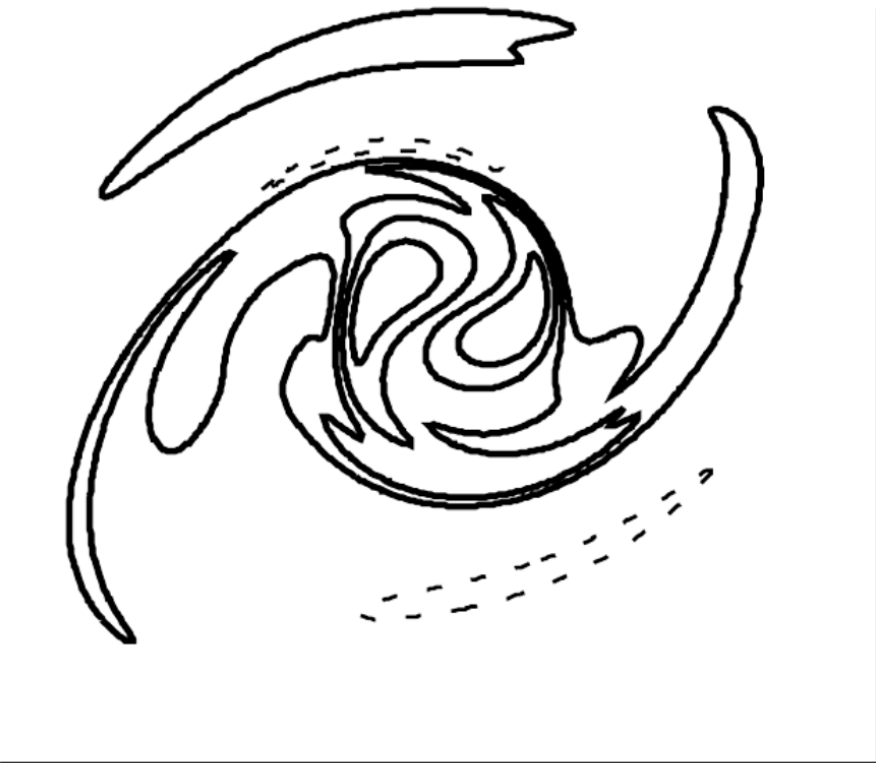
\includegraphics[width=0.225\textwidth]{figures/golanski2005-t182}
  \end{tabular}
\end{frame}
\begin{frame}
  \frametitle{Testcases}
  \framesubtitle{2D Non-Isothermal Mixing Layer - Results (Density)\subrule}

  \begin{tabular}{c c c c}
    % constcoeff - varcoeff-rho0 - varcoeff-rhoh - Golanski2005
    \textbf{CC} & \textbf{VC $\density_0$} & \textbf{VC $\density_h$} & \textbf{G2005} \\
    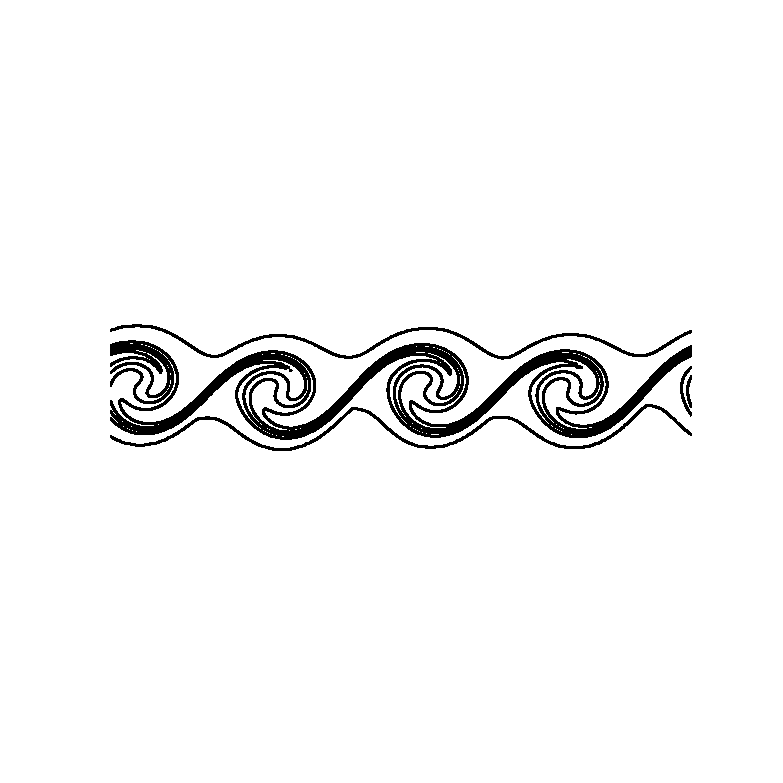
\includegraphics[width=0.2\textwidth]{figures/constcoeff-rho-024} & 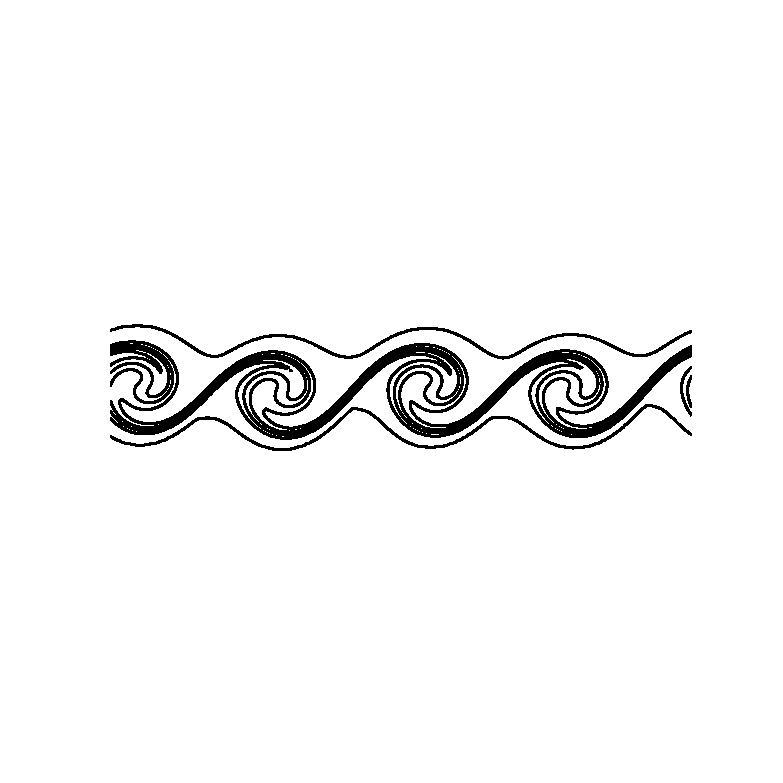
\includegraphics[width=0.2\textwidth]{figures/varcoeff-rho0-rho-024} & 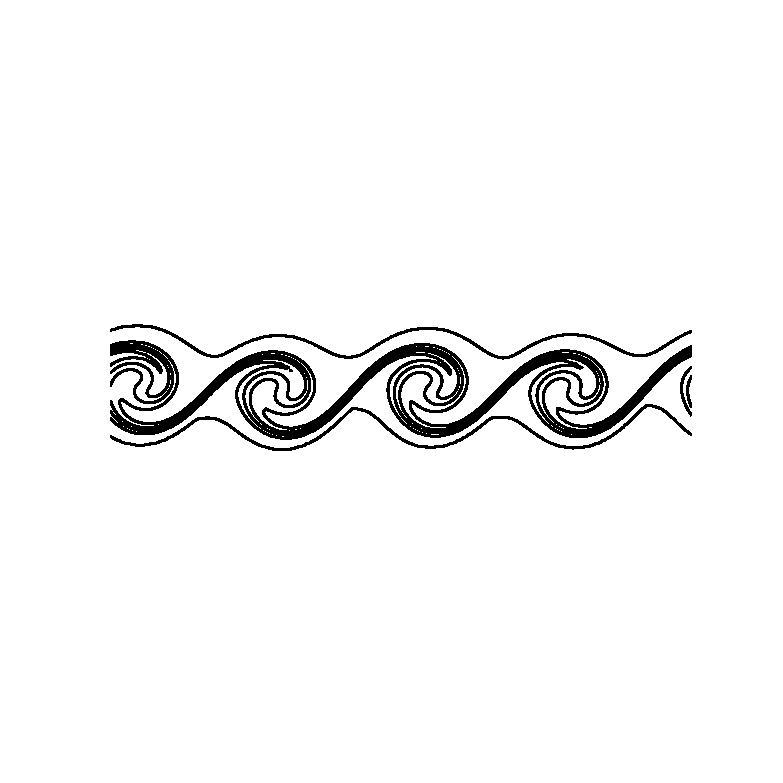
\includegraphics[width=0.2\textwidth]{figures/varcoeff-rhoh-rho-024} & 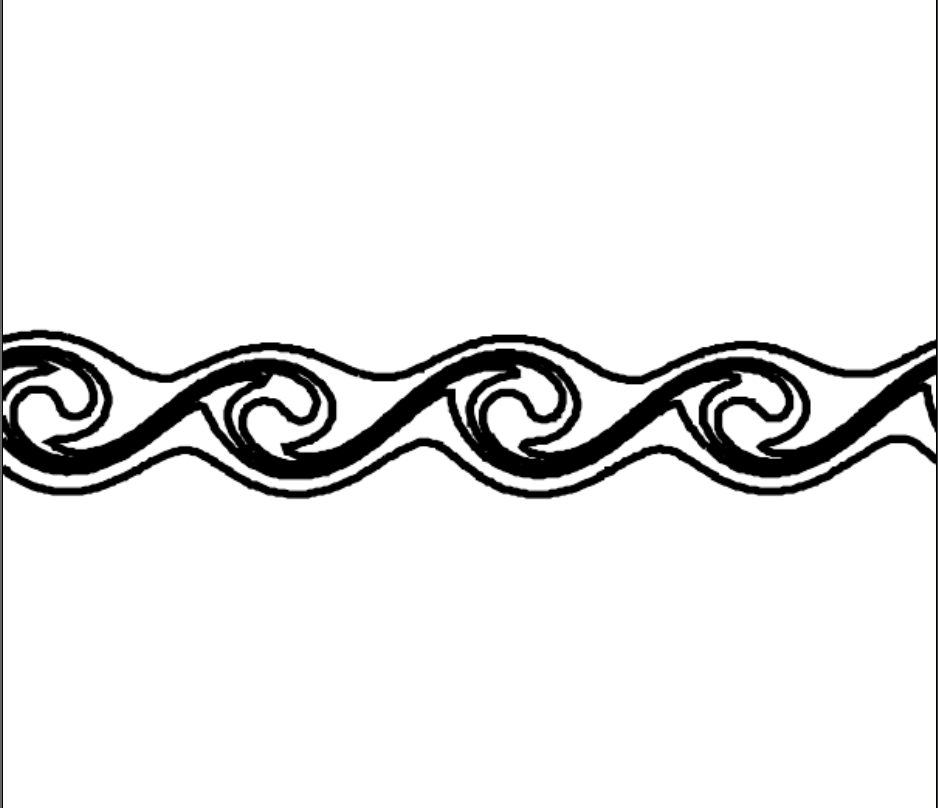
\includegraphics[width=0.2\textwidth]{figures/golanski2005-rho-t24}
    \\
    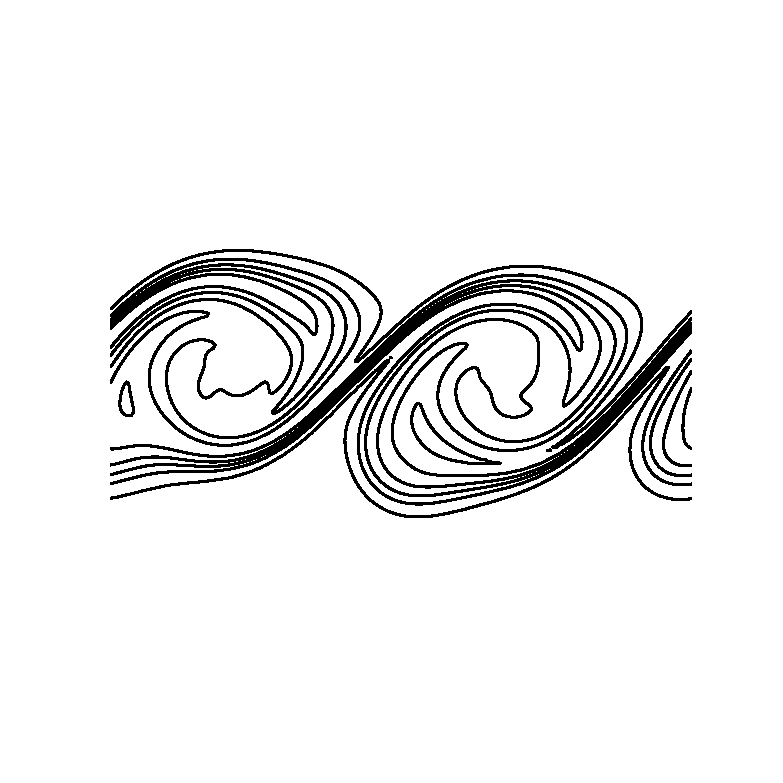
\includegraphics[width=0.2\textwidth]{figures/constcoeff-rho-082} & 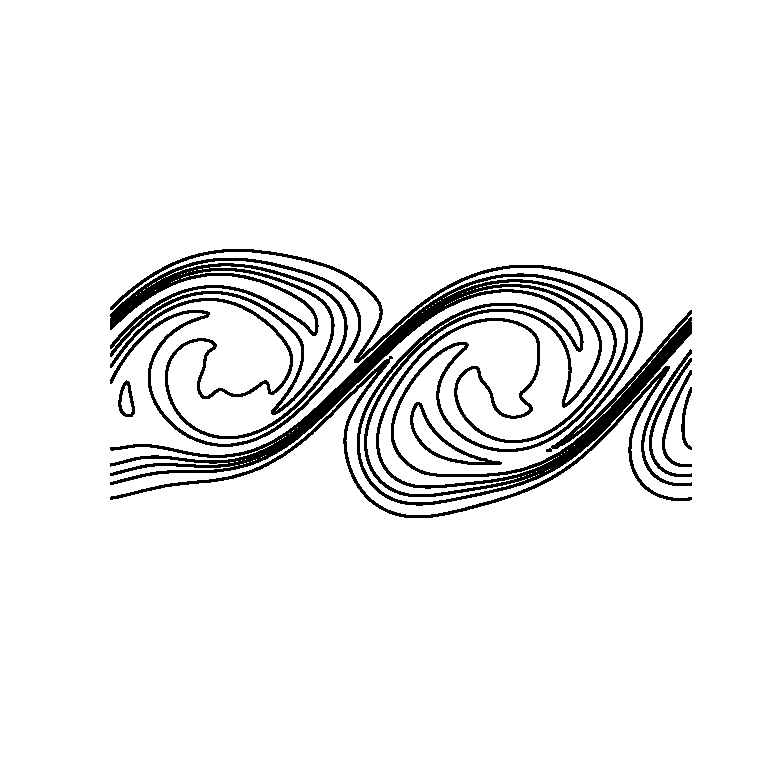
\includegraphics[width=0.2\textwidth]{figures/varcoeff-rho0-rho-082} & 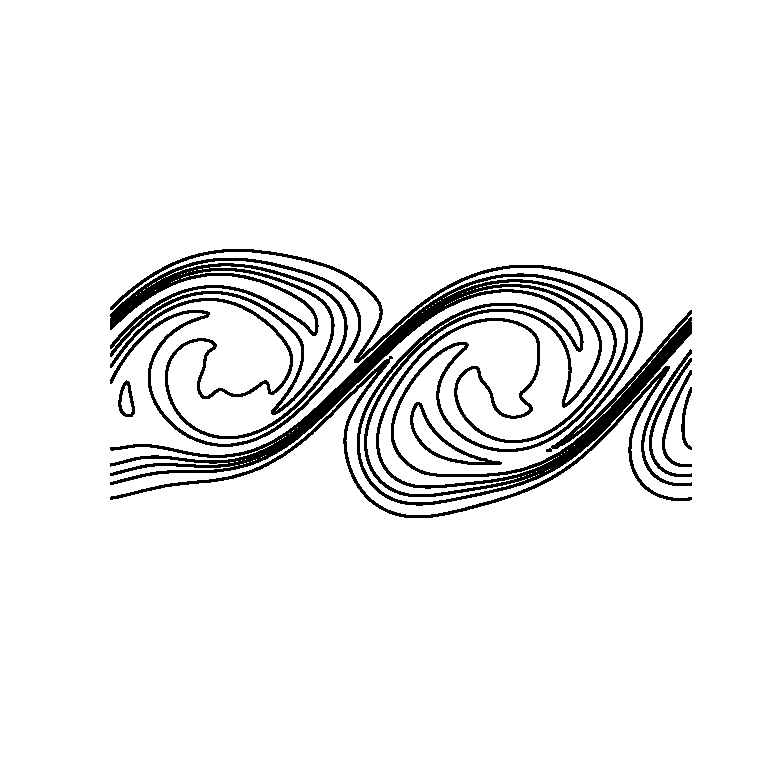
\includegraphics[width=0.2\textwidth]{figures/varcoeff-rhoh-rho-082} &
                                                                                       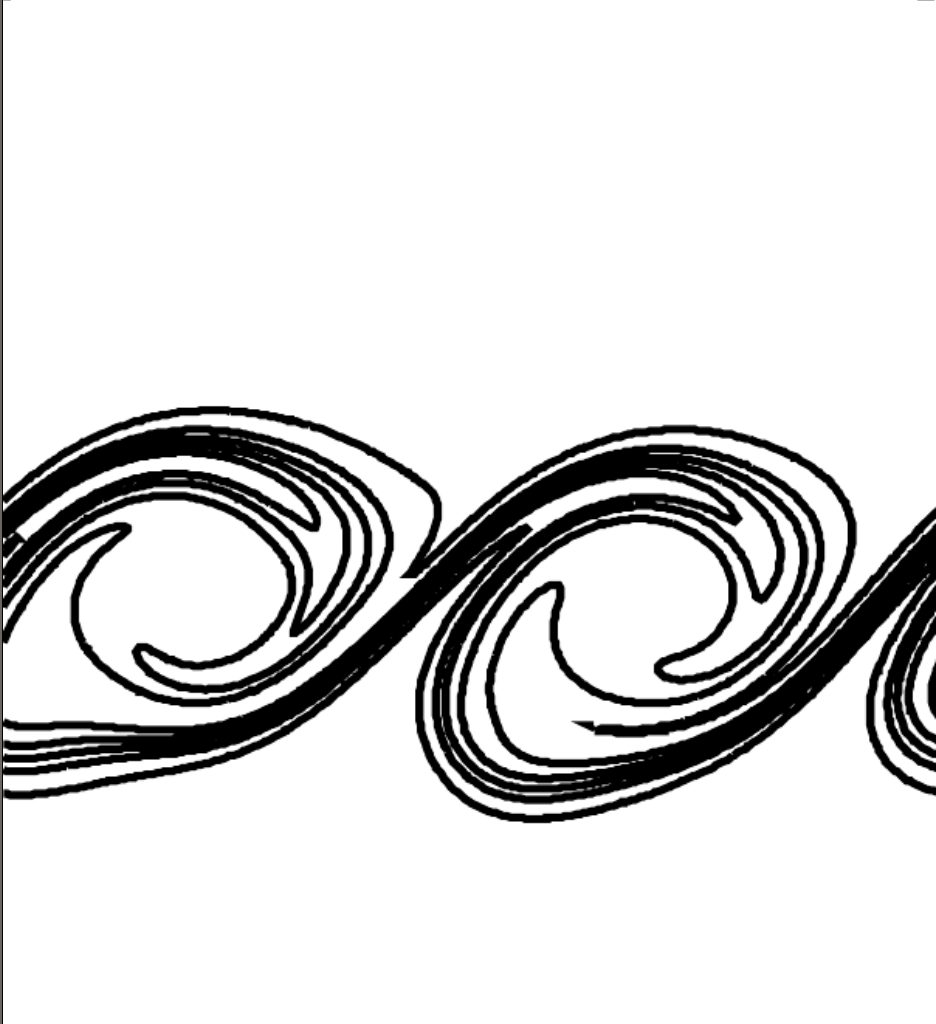
\includegraphics[width=0.2\textwidth]{figures/golanski2005-rho-t82} \\
    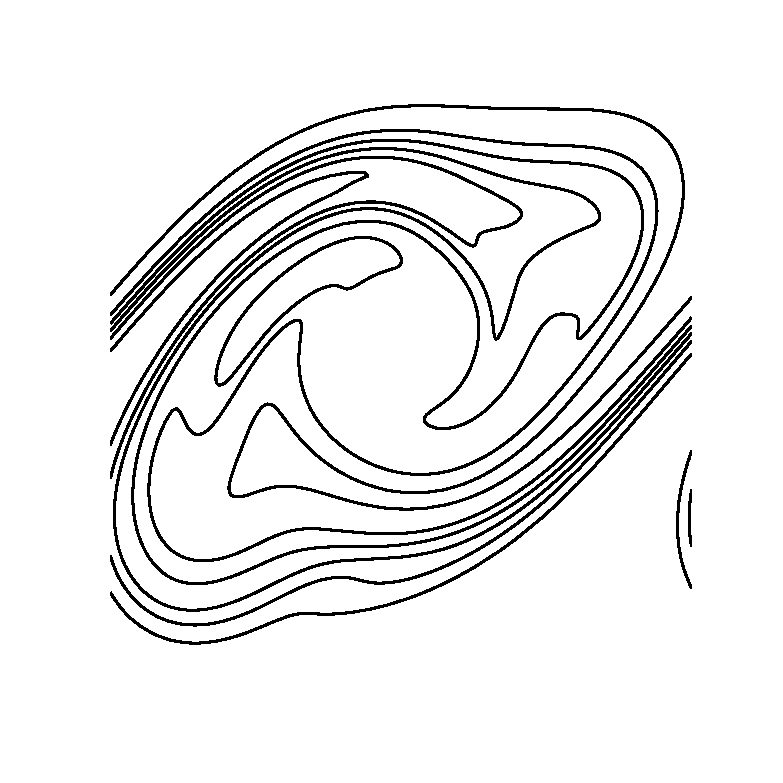
\includegraphics[width=0.2\textwidth]{figures/constcoeff-rho-182} & 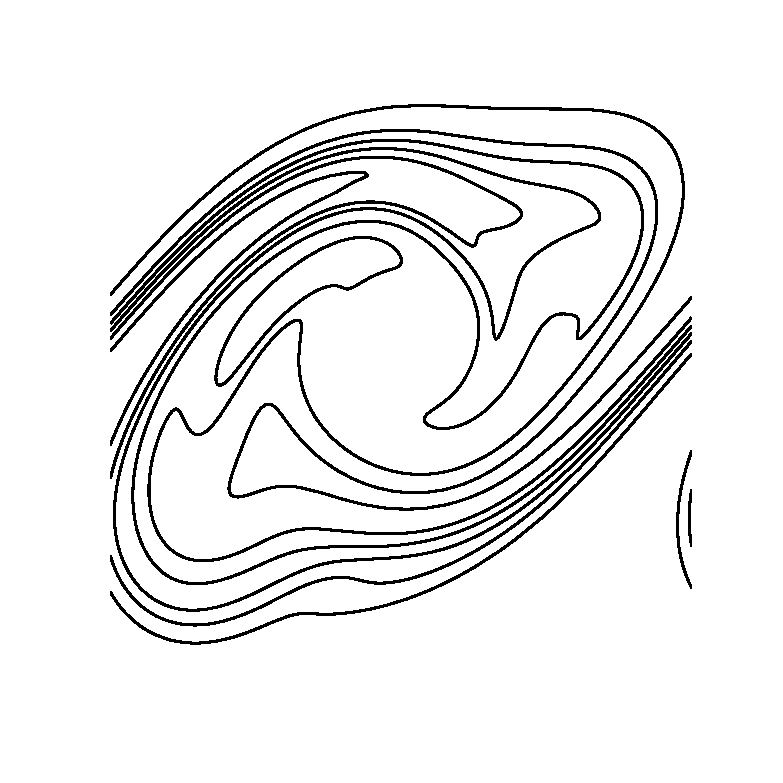
\includegraphics[width=0.2\textwidth]{figures/varcoeff-rho0-rho-182} & 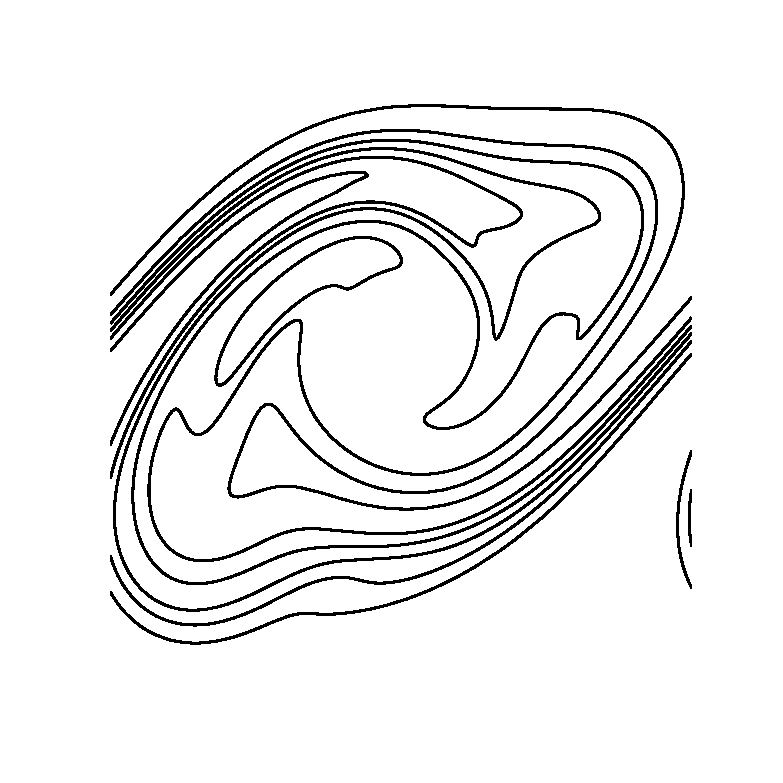
\includegraphics[width=0.2\textwidth]{figures/varcoeff-rhoh-rho-182} &
                                                                                       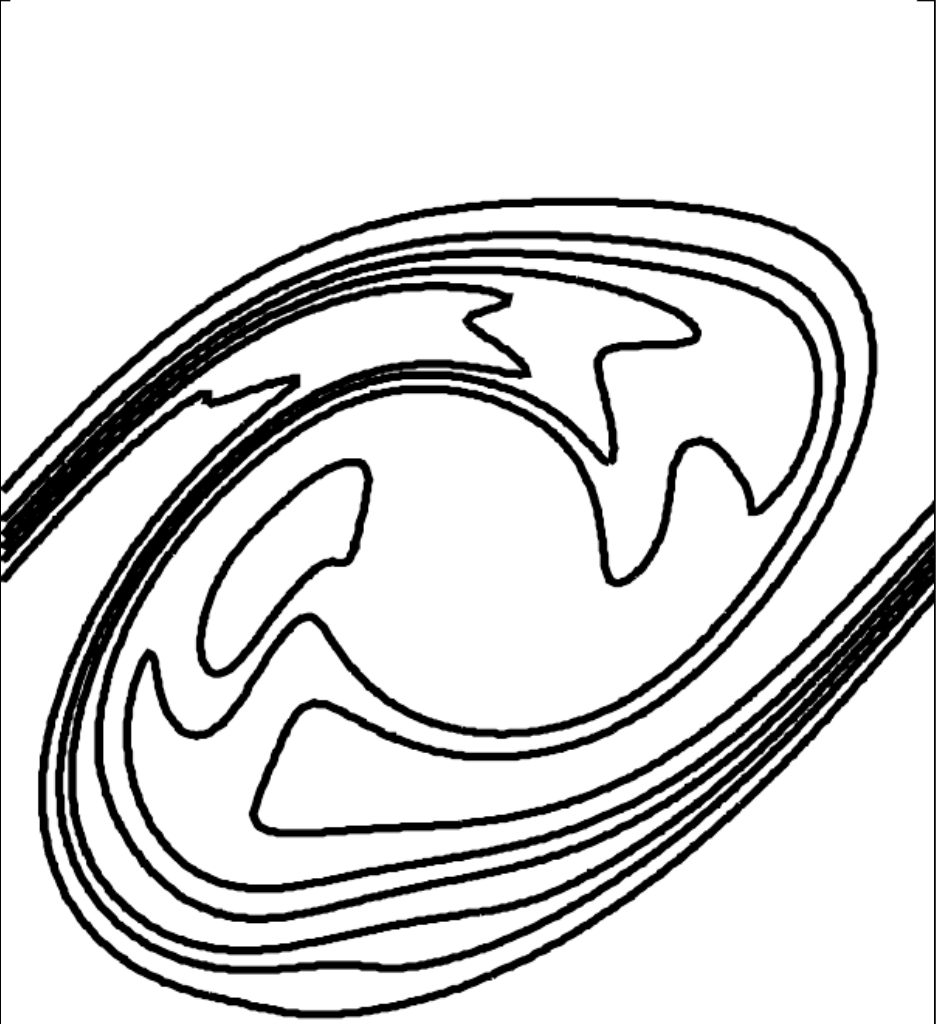
\includegraphics[width=0.2\textwidth]{figures/golanski2005-rho-t182}
  \end{tabular}
\end{frame}

\begin{frame}
  \frametitle{Testcases}
  \framesubtitle{2D Non-Isothermal Mixing Layer - Results (Error in $\vdiv{\vvelocity}^{k+1}$)\subrule}
  \begin{figure}[h]
    \centering
    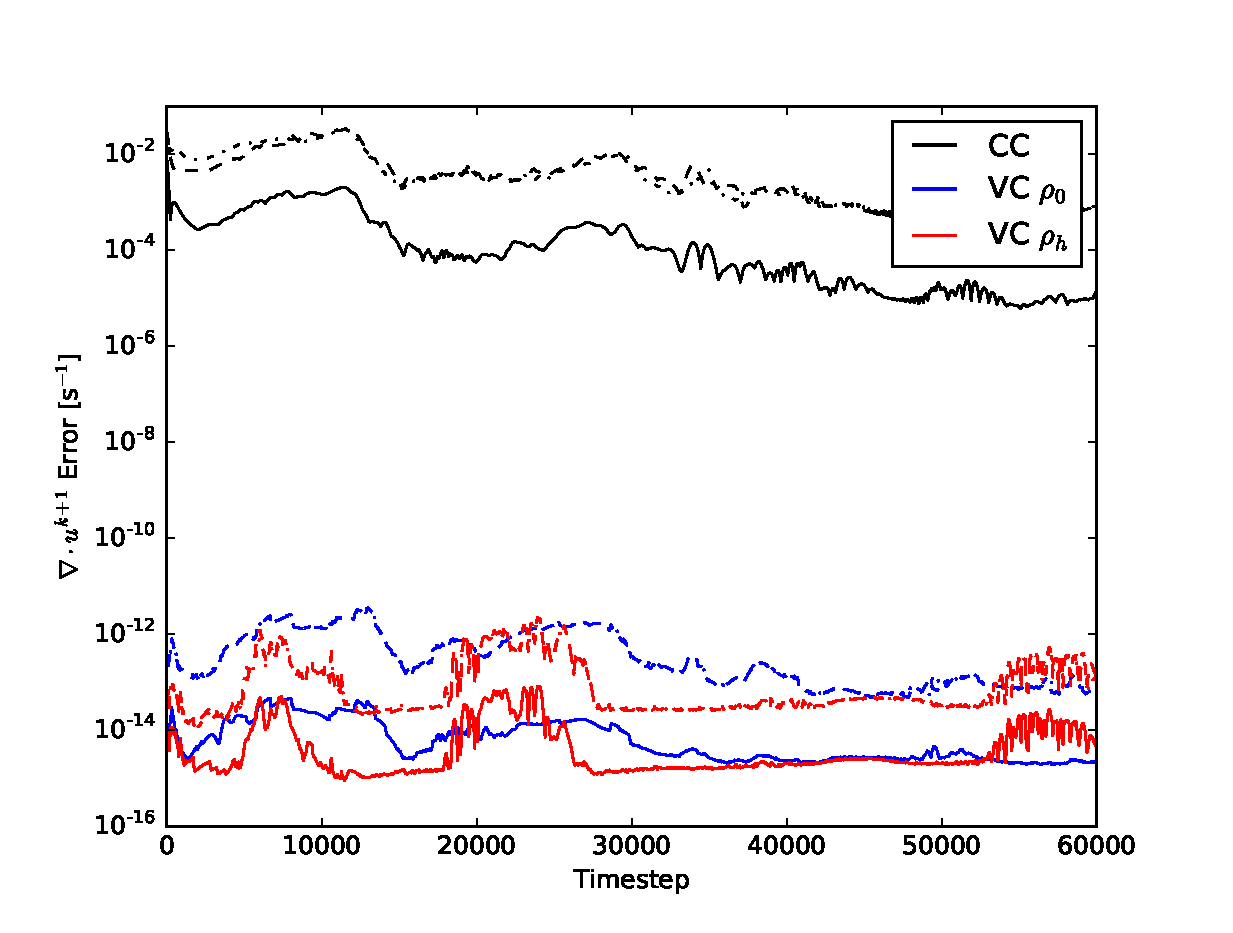
\includegraphics[width=0.95\textwidth]{figures/err_divu}
    % \caption{Error in divergence of corrected velocity field.}
  \end{figure}
\end{frame}

\begin{frame}
  \frametitle{Testcases}
  \framesubtitle{2D Non-Isothermal Mixing Layer - Results (Performance Comparison)\subrule}

  % \begin{columns}
  %   \begin{column}{0.5\textwidth}
  \begin{table}[h]
    \centering
    \begin{tabular}[h]{r | l}
      \textbf{Poisson Eq.} & \textbf{CPU / $\boldsymbol{\Delta t}$ [s]} \\
      \midrule
      CC & $4.48 \times 10^{-2}$ \\
      VC $\density_0$ & $6.16 \times 10^{-1}$ \\
      VC $\density_h$ & $3.53 \times 10^{-1}$ \\
      \midrule
                           & \textbf{Cost (normalised)} \\
      \midrule
      CC & $1$ \\
      VC $\density_0$ & $13.75$ \\
      VC $\density_h$ & $7.88$ \\
      \midrule
                           & \textbf{Time in Poisson [\%]} \\
      \midrule
      CC & $23.4$ ($1$) \\
      VC $\density_0$ & $94.2$ ($34.1$) \\
      VC $\density_h$ & $89.9$ ($18.8$)
    \end{tabular}
  \end{table}
  %   \end{column}
  %   \begin{column}{0.5\textwidth}
      
  %   \end{column}
  % \end{columns}
\end{frame}

% \begin{frame}
%   \frametitle{Testcases}
%   \framesubtitle{2D Non-Isothermal Mixing Layer - Discussion\subrule}
% \end{frame}

% Jet flow
\begin{frame}
  \frametitle{Testcases}
  \framesubtitle{Jet\subrule}

  \begin{columns}
    \begin{column}{0.5\textwidth}
      \begin{itemize}
      \item Jet is heated above ambient ($\temperature_j = 568\ K,\ \temperature_a = 300\ K$)
      % \item Small co-flow ($0.1$\% of $u_j$) for numerical stability
      \item Convective outflow boundary condition, convecting velocity chosen to satisfy
        \begin{equation*}
          \begin{split}
            \dtrans{\pressure^{\left( 0 \right)}} &= 0 \\
            \Rightarrow \int_{\partial \Omega} \vvelocity \cdot \widehat{\vvect{n}} dS &=
            \frac{\int_{\partial \Omega} k \vgrad{\temperature} \cdot \widehat{\vvect{n}}
              dS}{p^{\left( 0 \right)} \Reynolds \Prandtl}
          \end{split}
        \end{equation*}
      \item Free-slip applied at lateral boundaries
      \end{itemize}
    \end{column}
    \begin{column}{0.45\textwidth}
      \begin{figure}
        \centering
        %%% jet.tex --- 
%% 
%% Filename: jet.tex
%% Description: 
%% Author: Paul Bartholomew
%% Maintainer: 
%% Created: Mon Mar 12 14:45:53 2018 (+0000)
%% Version: 
%% Package-Requires: ()
%% Last-Updated: Mon Mar 26 16:13:15 2018 (+0100)
%%           By: Paul Bartholomew
%%     Update #: 62
%% URL: 
%% Doc URL: 
%% Keywords: 
%% Compatibility: 
%% 
%%%%%%%%%%%%%%%%%%%%%%%%%%%%%%%%%%%%%%%%%%%%%%%%%%%%%%%%%%%%%%%%%%%%%%
%% 
%%% Commentary: 
%% 
%% 
%% 
%%%%%%%%%%%%%%%%%%%%%%%%%%%%%%%%%%%%%%%%%%%%%%%%%%%%%%%%%%%%%%%%%%%%%%
%% 
%%% Change Log:
%% 
%% 
%%%%%%%%%%%%%%%%%%%%%%%%%%%%%%%%%%%%%%%%%%%%%%%%%%%%%%%%%%%%%%%%%%%%%%
%% 
%% This program is free software: you can redistribute it and/or modify
%% it under the terms of the GNU General Public License as published by
%% the Free Software Foundation, either version 3 of the License, or (at
%% your option) any later version.
%% 
%% This program is distributed in the hope that it will be useful, but
%% WITHOUT ANY WARRANTY; without even the implied warranty of
%% MERCHANTABILITY or FITNESS FOR A PARTICULAR PURPOSE.  See the GNU
%% General Public License for more details.
%% 
%% You should have received a copy of the GNU General Public License
%% along with GNU Emacs.  If not, see <http://www.gnu.org/licenses/>.
%% 
%%%%%%%%%%%%%%%%%%%%%%%%%%%%%%%%%%%%%%%%%%%%%%%%%%%%%%%%%%%%%%%%%%%%%%
%% 
%%% Code:

\resizebox{\columnwidth}{!}
{
  \begin{tikzpicture}
    \begin{axis}[
      xmin = -2, xmax = 2,
      ymin = -1, ymax = 8,
      axis lines = center,
      xlabel = $r$,
      ylabel = $y$,
      xticklabels={,,},
      yticklabels={,,}
      ]

      % Inlet velocity
      \addplot [mark=none, samples=200]
      {0.5 * (1 - tanh(2.5 * (2 * \x*\x - 1 / (2 * \x*\x))))};
      \draw [->] (axis cs: 0.6, 0) -- (axis cs: 0.6, 1);
      \draw [->] (axis cs: 0.4, 0) -- (axis cs: 0.4, 1);
      \draw [->] (axis cs: 0.2, 0) -- (axis cs: 0.2, 1);
      \draw [->] (axis cs: 0, 0) -- (axis cs: 0, 1);
      \draw [->] (axis cs: -0.6, 0) -- (axis cs: -0.6, 1);
      \draw [->] (axis cs: -0.4, 0) -- (axis cs: -0.4, 1);
      \draw [->] (axis cs: -0.2, 0) -- (axis cs: -0.2, 1);

      % Illustration of spreading
      \draw [dashed] (axis cs: 1, 0) -- (axis cs: 1.75, 8);
      \draw [dashed] (axis cs: -1, 0) -- (axis cs: -1.75, 8);

      \draw [<->] (axis cs: -1, -0.5) -- (axis cs: 1, -0.5);
      \node at (axis cs: 1.2, -0.5) {$D$};

      % % Gravity vector
      % \draw [->] (axis cs: 0.5, 6) -- (axis cs: 0.5, 4);
      % \node at (axis cs: 0.7, 5) {$g$};

      % Density
      \node at (axis cs: -0.5, 2) {$\density_j$};
      \node at (axis cs: -1.5, 1) {$\density_a$};

      % % Sponge
      % \fill[black!40!white, opacity=0.2] (axis cs: -2, 7) rectangle (axis cs: 2, 8);
      % \node at (axis cs: -1, 7.5) {`Sponge'};
    \end{axis}
  \end{tikzpicture}
}

%%%%%%%%%%%%%%%%%%%%%%%%%%%%%%%%%%%%%%%%%%%%%%%%%%%%%%%%%%%%%%%%%%%%%%
%%% jet.tex ends here

%%% Local Variables:
%%% mode: latex
%%% TeX-master: "../pres_quasincompact3d"
%%% End:

        \caption{Diagram of jet}\label{fig:jet}
      \end{figure}
    \end{column}
  \end{columns}
\end{frame}
\begin{frame}
  \frametitle{Testcases}
  \framesubtitle{Jet - Results\subrule}

  % % media9
  % \includemedia[activate=pageopen,
  % height=\textheight]{}{./figures/vort.ogv}

  % % movie15
  % \includemovie[]{}{}{./figures/vort.mp4}

  % multimedia
    \movie[
    height=0.6\textheight,
    width=\textwidth,
    poster,
    autostart
    ]{}{./figures/vort.ogv}
\end{frame}

%%%%%%%%%%%%%%%%%%%%%%%%%%%%%%%%%%%%%%%%%%%%%%%%%%%%%%%%%%%%%%%%%%%%%%
% Conclusion
\begin{frame}
  \frametitle{Conclusion and Future Work}
  \framesubtitle{\ \subrule}

  \begin{columns}
    \begin{column}{0.5\textwidth}
      \begin{itemize}
      \item LMN implemented in \incompact
      \item Implemented constant and variable coefficient Poisson solvers
      \item Proposed new formulation for variable coefficient Poisson solver
      \end{itemize}
    \end{column}
    \begin{column}{0.5\textwidth}
      \begin{itemize}
      \item Complete simulation of buoyant, turbulent jets
      \item Multicomponent flows
      \end{itemize}
    \end{column}
  \end{columns}

  \vfill

  \centering
  \huge{Thanks for listening!}
%   \begin{figure}
%     \centering
%     \begin{subfigure}
%       \centering
%       
\includegraphics[width=0.25\textwidth]{./figures/imperial}
%     \end{subfigure}
%     \hfill
%     \begin{subfigure}
%       \centering
%       
\includegraphics[width=0.25\textwidth]{./figures/epsrc}
%     \end{subfigure}
%     \hfill
%     \begin{subfigure}
%       \centering
%       
\includegraphics[width=0.25\textwidth]{./figures/archer}
%     \end{subfigure}
%   \end{figure}
\end{frame}

\begin{frame}<beamer:0> % Suppress references page
  \bibliographystyle{natbib}
  \bibliography{/home/paul/Documents/Postdoc.bib}
\end{frame}
\end{document}

%%%%%%%%%%%%%%%%%%%%%%%%%%%%%%%%%%%%%%%%%%%%%%%%%%%%%%%%%%%%%%%%%%%%%%
%%% pres_quasincompact3d.tex ends here

%%% Local Variables:
%%% mode: latex
%%% TeX-master: t
%%% End:
